%%%%%%%%%%%%%%%%%%%%%%%%%%%%%%%% COMMENT THIS TO COMPILE main.tex %%%%%%%%%%%%%%%%%%%%%%%%%%%%%%%%
\documentclass[a4paper,12pt]{report}
\documentclass[a4paper,12pt]{report}
\usepackage[english]{babel}
\usepackage[left=2cm,right=2cm,top=2cm,bottom=2cm]{geometry}
%\usepackage{mathtools}
\usepackage{amsthm}     % for definitions and theorems
\usepackage[many]{tcolorbox}    % boxes around definitions and theorems
%\usepackage{amsmath}
%\usepackage{nccmath}
\usepackage{amssymb}    % \ltimes
\usepackage{etoolbox}   % for start of Chapter
%\usepackage{amsfonts}
\usepackage{physics}    % for all Physics related
\usepackage{dsfont}     % for the identity matrix symbol \1
%\usepackage{mathrsfs}

\usepackage{titling}
\usepackage{indentfirst}

\usepackage{bm}
\usepackage[dvipsnames]{xcolor}
\usepackage{cancel}

\usepackage{xurl}
\usepackage[colorlinks=true]{hyperref}

\usepackage{float}
\usepackage{graphicx}
\usepackage{subcaption}
%\usepackage{tikz}

\usepackage{ctable}     % tabelas
\renewcommand{\P}{\phantom{+}}  % empty space to indent things
\usepackage{multirow}
\usepackage{tabulary}

%%%%%%%%%%%%%%%%%%%%%%%%%%%%%%%%%%%%%%%%%%%%%%%%%%%

\newcommand{\eps}{\epsilon}
\newcommand{\vphi}{\varphi}
\newcommand{\cte}{\text{cte}}

\newcommand{\N}{{\mathbb{N}}}
\newcommand{\Z}{{\mathbb{Z}}}
%\newcommand{\Q}{{\mathbb{Q}}}
\newcommand{\C}{{\mathbb{C}}}
\renewcommand{\S}{{\hat{S}}}
%\renewcommand{\H}{\s{H}}

\renewcommand{\a}{{\vb{a}}}
\renewcommand{\b}{{\vb{b}}}
\renewcommand{\d}{{\dagger}}
\newcommand{\up}{{\uparrow}}
\newcommand{\down}{{\downarrow}}
\newcommand{\hc}{{\text{h.c.}}}

\newcommand{\ihat}{\bm{\hat{\imath}}}
\newcommand{\jhat}{\bm{\hat{\jmath}}}
\newcommand{\khat}{\bm{\hat{k}}}

\newcommand{\0}{{\vb{0}}}
\newcommand{\1}{\mathds{1}}
\newcommand{\E}{{\vb{E}}}
\newcommand{\B}{{\vb{B}}}
\renewcommand{\u}{{\vb{u}}}
\renewcommand{\v}{{\vb{v}}}
\renewcommand{\r}{{\vb{r}}}
\newcommand{\R}{{\vb{R}}}
\newcommand{\Q}{{\vb{Q}}}
\newcommand{\G}{{\vb{G}}}
\newcommand{\g}{{\vb{g}}}
\renewcommand{\k}{{\vb{k}}}
\newcommand{\K}{{\vb{K}}}
\newcommand{\p}{{\vb{p}}}
\newcommand{\q}{{\vb{q}}}
\newcommand{\F}{{\vb{F}}}
\renewcommand{\t}{{\vb{t}}}
\newcommand{\vtau}{{\bm{\tau}}}
\newcommand{\vdelta}{{\bm{\delta}}}

% COLORED SYMMETRY ELEMENTS
\newcommand{\Ct}{{\textcolor{Cyan}{C_3}}}
\newcommand{\Ctn}[1]{{\textcolor{Cyan}{C_3^{\textcolor{black}{#1}}}}}
\newcommand{\Cs}{{\textcolor{ForestGreen}{C_6}}}
\newcommand{\Csn}[1]{{\textcolor{ForestGreen}{C_6^{\textcolor{black}{#1}}}}}
\newcommand{\sd}{{\textcolor{RoyalBlue}{\sigma_d}}}
\newcommand{\sdn}[1]{{\textcolor{RoyalBlue}{\sigma_d^{\textcolor{black}{#1}}}}}
\newcommand{\sdp}{{\textcolor{RoyalBlue}{\sigma_d'}}}
\newcommand{\sdpp}{{\textcolor{RoyalBlue}{\sigma_d''}}}
\newcommand{\sv}{{\textcolor{Orange}{\sigma_v}}}
\newcommand{\svn}[1]{{\textcolor{Orange}{\sigma_v^{\textcolor{black}{#1}}}}}
\newcommand{\svp}{{\textcolor{Orange}{\sigma_v'}}}
\newcommand{\svpp}{{\textcolor{Orange}{\sigma_v''}}}

\newcommand{\s}{\sigma}
%\newcommand{\prodint}[2]{\left\langle #1 , #2 \right\rangle}
\newcommand{\cc}[1]{\overline{#1}}
\newcommand{\Eval}[3]{\eval{\left( #1 \right)}_{#2}^{#3}}
\newcommand{\sg}[2]{\{ #1 \mid #2 \}}

\newcommand{\unit}[1]{\; \mathrm{#1}}

\newcommand{\n}{\medskip}
\newcommand{\e}{\quad \mathrm{and} \quad}
\newcommand{\ou}{\quad \mathrm{or} \quad}
\newcommand{\virg}{\, , \;}
\newcommand{\ptodo}{\forall \,}
\renewcommand{\implies}{\; \Rightarrow \;}
%\newcommand{\eqname}[1]{\tag*{#1}} % Tag equation with name

\setlength{\droptitle}{-7em}

\makeatletter
\patchcmd{\chapter}{\if@openright\cleardoublepage\else\clearpage\fi}{}{}{}  % start 'Chapter' at the same page. needs package etoolbox
\makeatother

%% Theorems, definitions, proofs
\theoremstyle{definition}

\newtheorem{definition}{Definition}[section]
\tcolorboxenvironment{definition}{
  colback=blue!5!white,
  boxrule=0pt,
  boxsep=1pt,
  left=2pt,right=2pt,top=2pt,bottom=2pt,
  oversize=2pt,
  sharp corners,
  before skip=\topsep,
  after skip=\topsep,
}

\newtheorem{theorem}{Theorem}[section]
\tcolorboxenvironment{theorem}{
  colback=blue!5!white,
  boxrule=0pt,
  boxsep=1pt,
  left=2pt,right=2pt,top=2pt,bottom=2pt,
  oversize=2pt,
  sharp corners,
  before skip=\topsep,
  after skip=\topsep,
}

\begin{document}
%%%%%%%%%%%%%%%%%%%%%%%%%%%%%%%% COMMENT THIS TO COMPILE main.tex %%%%%%%%%%%%%%%%%%%%%%%%%%%%%%%%


%%%%%%%%%%%%%%%%%%%%%%%%%%%%%%%%%%%%%%%%%%%%%%%%%%%%%%%%%%%%%%%%%%%%%%%%%%%%%%%%%%%%%%%%%%%%%%%%%%
\chapter{Emergent symmetries in Twisted Bilayer Graphene}
%%%%%%%%%%%%%%%%%%%%%%%%%%%%%%%%%%%%%%%%%%%%%%%%%%%%%%%%%%%%%%%%%%%%%%%%%%%%%%%%%%%%%%%%%%%%%%%%%%

\section{Space Groups}

Here we are going to study the concept of \textit{space groups}. It is very important to classify the symmetry properties of the system in interest (Twisted Bilayer Graphene). In our examples, we are going to focus on the familiar honeycomb lattice example. The space group is loosely an semi-direct product of the point group and the translation group. Given a fixed lattice, all the linear transformations that carry the lattice into itself belong to the space group. A useful matrix representation for $G$ is:
\begin{equation} \label{eq:spacegroup-rep}
\sg{R_\alpha}{\vtau} =
\begin{pmatrix}
1 & 0 \\
\vtau & R_\alpha
\end{pmatrix},
\end{equation}
where $0$ is a row of three zeros, $\vtau$ is a column vector and $R_\alpha$ is $3\times 3$ rotation matrix.

The inverse of an element is given by
\begin{equation} \label{eq:inv-spacegroup}
\sg{R_\alpha}{\vtau}^{-1} =
\begin{pmatrix}
1 & 0 \\
-R_\alpha^{-1}\vtau & R_\alpha^{-1}
\end{pmatrix} =
\sg{R_\alpha^{-1}}{-R_\alpha^{-1}\vtau}.
\end{equation}

Let's take the honeycomb lattice as the example. The space group of interest $P622$ \cite{thesis_rennella} is symmorphic (Table 9.1 of \cite{dresselhaus}). Therefore it is impossible to find a screw axis or glide plane. We have to rely on pure translation + pure point group.

\textbf{IT IS MUCH BETTER TO MAKE THE EXAMPLE 2x2}

For example, let's take a translation of $d(\cos30^\circ, \sin30^\circ)$ with a rotation of $60^\circ$. The result is
$$
\begin{pmatrix}
1 & 0 & 0 & 0 \\
\frac{a}{2} & \frac{1}{2} & \frac{\sqrt{3}}{2} & 0 \\
\frac{a\sqrt{3}}{6} & -\frac{\sqrt{3}}{2} & \frac{1}{2} & 0 \\
0 & 0 & 0 & 1 \\
\end{pmatrix}
$$

Some arbitrary lattice vector is represented by (the basis is $(0, b)$, where $b = 0$ or $b = \frac{2a}{\sqrt{3}}$).
$$
\begin{pmatrix} 1 \\
m\begin{pmatrix} \frac{a}{2} \\ \frac{a\sqrt{3}}{2} \\ 0 \end{pmatrix} + n \begin{pmatrix} -\frac{a}{2} \\ \frac{a\sqrt{3}}{2} \\ 0 \end{pmatrix} + \begin{pmatrix} 0 \\ b \\ 0 \end{pmatrix}
\end{pmatrix}
=
\begin{pmatrix}
1 \\ (m-n)\frac{a}{2} \\ (m+n)\frac{a\sqrt{3}}{2} + b \\ 0
\end{pmatrix}
$$

\n

$$
\begin{pmatrix}
1 & 0 & 0 & 0 \\
\frac{a}{2} & \frac{1}{2} & \frac{\sqrt{3}}{2} & 0 \\
\frac{a\sqrt{3}}{6} & -\frac{\sqrt{3}}{2} & \frac{1}{2} & 0 \\
0 & 0 & 0 & 1 \\
\end{pmatrix}
\begin{pmatrix}
1 \\ (m-n)\frac{a}{2} \\ (m+n)\frac{a\sqrt{3}}{2} + b \\ 0
\end{pmatrix}
=
\begin{pmatrix}
1 \\ (2m-n+1)\frac{a}{2} + \qty(\frac{\sqrt{3}b}{2}) \\ n \frac{a\sqrt{3}}{2} + \qty(\frac{a\sqrt{3}}{6} + \frac{b}{2}) \\ 0
\end{pmatrix}
$$

\n

\textbf{Example of nonsymmorphic space group}: Tellurium screw axis $3_1$. Glide plane triangular lattice, translation $a/2$ and reflection.



+++++++++++++++++++++++++++++++++++++++++++++++
\section{ABAIXO DISSO É COISA ANTIGA}
+++++++++++++++++++++++++++++++++++++++++++++++

%%%%%%%%%%%%%%%%%%%%%%%%%%%%%%%%%%%%%%%%%%%%%%%%%%%%%%%%%%%%%%%%%%%%%%%%%%%%%%%%%%%%%%%%%%%%%%%%%%
\section{Elements of group theory}
%%%%%%%%%%%%%%%%%%%%%%%%%%%%%%%%%%%%%%%%%%%%%%%%%%%%%%%%%%%%%%%%%%%%%%%%%%%%%%%%%%%%%%%%%%%%%%%%%%

%%%%%%%%%%%%%%%%%%%%%%%%%%%%%%%%%%%%%%%%%%%%%%%%%%%%%%%%%%%%%%%%%%%%%%%%%%%%%%%%%%%%%%%%%%%%%%%%%%
\subsection{Cosets}
%%%%%%%%%%%%%%%%%%%%%%%%%%%%%%%%%%%%%%%%%%%%%%%%%%%%%%%%%%%%%%%%%%%%%%%%%%%%%%%%%%%%%%%%%%%%%%%%%%

Given a subgroup $H$ (order $\abs{H}$) of a group $G$ (order $\abs{G}$), and an element $g \in G$, we define the left coset $gH$ by
$$
gH = \{gh \mid h \in H\} \subseteq G.
$$

We know from Laplace's theorem that every left coset has the same number of elements $\abs{G:H} = \abs{G} / \abs{H}$, which is called the \textit{index} of $H$, and $G$ is a disjoint union of its left cosets:
$$
G = \sum_{j=1}^{\abs{G:H}} g_i H,
$$
where $g_i \in G$ are representatives of the left cosets $g_i H$.

%%%%%%%%%%%%%%%%%%%%%%%%%%%%%%%%%%%%%%%%%%%%%%%%%%%%%%%%%%%%%%%%%%%%%%%%%%%%%%%%%%%%%%%%%%%%%%%%%%
\subsection{Conjugacy classes}
%%%%%%%%%%%%%%%%%%%%%%%%%%%%%%%%%%%%%%%%%%%%%%%%%%%%%%%%%%%%%%%%%%%%%%%%%%%%%%%%%%%%%%%%%%%%%%%%%%

An element $g' = a g a^{-1}$ is the \textit{conjugate} element of $g$ by means of $a$, and we write $g' \sim g$. This forms a conjugacy relation, and
$$
[g] = \{a g a^{-1} \mid a \in G\}
$$
is called a conjugacy class. The group $G$ is a disjoint union of its conjugacy classes.

%%%%%%%%%%%%%%%%%%%%%%%%%%%%%%%%%%%%%%%%%%%%%%%%%%%%%%%%%%%%%%%%%%%%%%%%%%%%%%%%%%%%%%%%%%%%%%%%%%
\subsection{Normal subgroup}
%%%%%%%%%%%%%%%%%%%%%%%%%%%%%%%%%%%%%%%%%%%%%%%%%%%%%%%%%%%%%%%%%%%%%%%%%%%%%%%%%%%%%%%%%%%%%%%%%%

If $H \leq G$, we say that $H$ is a normal subgroup of $G$ if $g H g^{-1} = H$ for every $g \in G$.

One commom example of normal subgroup is
$$
G = \{ \text{invertible matrices} \},
$$
$$
H = \{ \text{matrices of determinant 1} \}.
$$

%%%%%%%%%%%%%%%%%%%%%%%%%%%%%%%%%%%%%%%%%%%%%%%%%%%%%%%%%%%%%%%%%%%%%%%%%%%%%%%%%%%%%%%%%%%%%%%%%%
\subsection{Homomorphism and Isomorphism}
%%%%%%%%%%%%%%%%%%%%%%%%%%%%%%%%%%%%%%%%%%%%%%%%%%%%%%%%%%%%%%%%%%%%%%%%%%%%%%%%%%%%%%%%%%%%%%%%%%

If $G$ and $H$ are groups, and $\vphi: G \to H$ is a function that satisfies
$$
\vphi(a)\vphi(b) = \vphi(ab), \quad \ptodo a,b \in G,
$$
then we say that $\vphi$ is a homomorphism between $G$ and $H$. If $\vphi$ is bijective, we say it is a isomorphism and that $G$ is isomorphic to $H$.

%%%%%%%%%%%%%%%%%%%%%%%%%%%%%%%%%%%%%%%%%%%%%%%%%%%%%%%%%%%%%%%%%%%%%%%%%%%%%%%%%%%%%%%%%%%%%%%%%%
\subsection{Induction and subduction of representations}
%%%%%%%%%%%%%%%%%%%%%%%%%%%%%%%%%%%%%%%%%%%%%%%%%%%%%%%%%%%%%%%%%%%%%%%%%%%%%%%%%%%%%%%%%%%%%%%%%%

Let us consider an irreducible representation $\Gamma$ of a group $G$. Now, given a subgroup $H$ of $G$, we can construct the so-called \textit{subduced} representation of $H$, formed by the matrices of those elements of $G$ that also belong to $H$, that is $\Gamma(h)$ for $h \in H$. This representation is in general reducible, and it is denoted by $\Gamma \downarrow H$.

Thinking in the other direction, if we start with an irreducible representation $D$ of $H \leq G$, we can construct the so-called \textit{induced} representation of $D \uparrow G = \Delta$ of $G$, as follows
\begin{align*}
\Delta_{i'j'ij}(g) =
\begin{cases}
\; D_{i'i}(g_{j'}^{-1} g g_j), \quad & g_{j'}^{-1} g g_j \in H, \\
\; 0,  & g_{j'}^{-1} g g_j \notin H.
\end{cases}
\end{align*}

%%%%%%%%%%%%%%%%%%%%%%%%%%%%%%%%%%%%%%%%%%%%%%%%%%%%%%%%%%%%%%%%%%%%%%%%%%%%%%%%%%%%%%%%%%%%%%%%%%
\section{Space Groups}
%%%%%%%%%%%%%%%%%%%%%%%%%%%%%%%%%%%%%%%%%%%%%%%%%%%%%%%%%%%%%%%%%%%%%%%%%%%%%%%%%%%%%%%%%%%%%%%%%%

The point group and translation symmetry operations which carry the crystel into itself form a group called the \textit{space group}. The elements of it are commonly denoted by  $\{ R_\alpha \mid \tau \} $, where $R_\alpha$ is the point group operation and $\tau$ is the translation.

Pure rotations and pure translations are special cases of space group operations:
\begin{itemize}
\item $\sg{\eps}{0} =$ identity.
\item $\sg{R_\alpha}{0} =$ pure point group operation.
\item $\sg{\eps}{\tau} =$ pure translation.
\end{itemize}

The result for the multiplication of two space group operations is
$$
\sg{R_\beta}{\tau_2} \sg{R_\alpha}{\tau_1} = \sg{R_\beta R_\alpha}{R_\beta\tau_1 + \tau_2}.
$$

Beyond pure operations, we may find compound operations that combine translations and point group operations. The two possible types are \textit{glide planes} and \textit{screw axes}.
\begin{figure}[H]
\centering
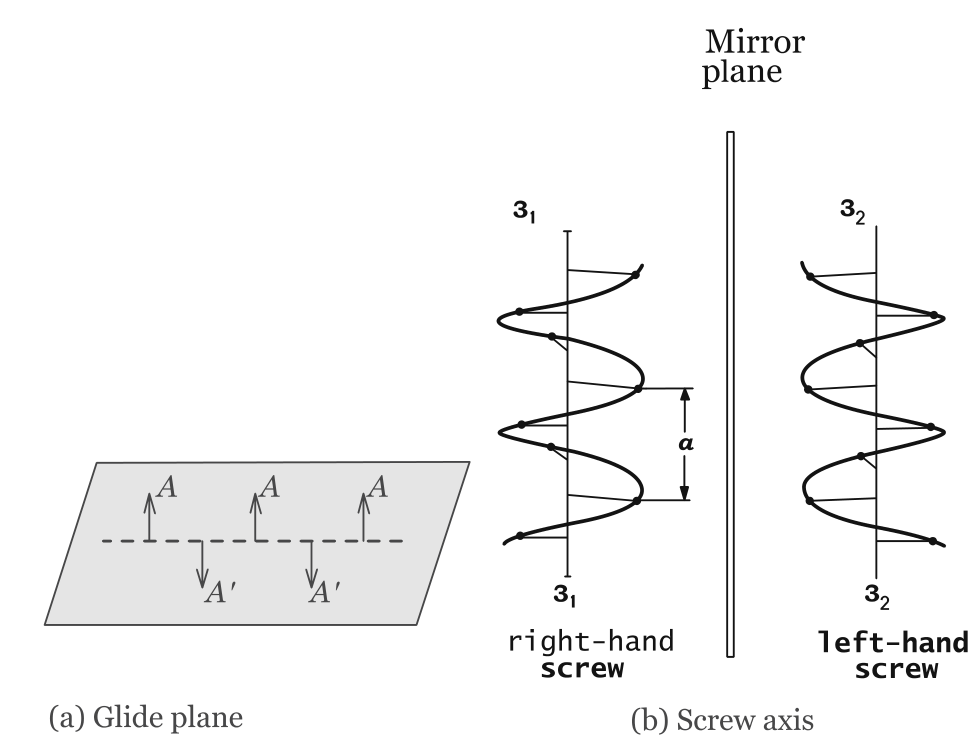
\includegraphics[width=0.5\linewidth]{fig/glideplane-screwaxis.png}
\caption{(a) The glide plane takes $A$ into $A'$. (b) Right- and left-hand screw axis.}
\label{fig:glideplane-screwaxis}
\end{figure}

%%%%%%%%%%%%%%%%%%%%%%%%%%%%%%%%%%%%%%%%%%%%%%%%%%%%%%%%%%%%%%%%%%%%%%%%%%%%%%%%%%%%%%%%%%%%%%%%%%
\subsection{Translation subgroup}
%%%%%%%%%%%%%%%%%%%%%%%%%%%%%%%%%%%%%%%%%%%%%%%%%%%%%%%%%%%%%%%%%%%%%%%%%%%%%%%%%%%%%%%%%%%%%%%%%%

All the elements $\sg{\eps}{\tau}$ of the the space group $G$ constitute the translation group $T$. It is a subgroup of $G$ and defines the Bravais lattice. More than that, $T$ is a normal subgroup of $G$, which means that $g T g^{-1} = T$ for every $g \in G$. Because of that, the cosets
$$
\{ \sg{R_\alpha}{\tau'} \sg{\eps}{\tau} \mid \sg{\eps}{\tau} \in T \} \in G/T
$$
form a factor group of the space group $G$.

This factor group $G/T$ is actually isomorphic to the point group of $G$.

%%%%%%%%%%%%%%%%%%%%%%%%%%%%%%%%%%%%%%%%%%%%%%%%%%%%%%%%%%%%%%%%%%%%%%%%%%%%%%%%%%%%%%%%%%%%%%%%%%
\subsection{Symmorphic and Nonsymmorphic Space Groups}
%%%%%%%%%%%%%%%%%%%%%%%%%%%%%%%%%%%%%%%%%%%%%%%%%%%%%%%%%%%%%%%%%%%%%%%%%%%%%%%%%%%%%%%%%%%%%%%%%%

In a space group $G$, we can always rewrite its elements in the form
$$
\sg{R_\alpha}{\tau} = \sg{R_\alpha}{r_n + \tau} = \sg{\eps}{r_n} \sg{R_\alpha}{\tau_\alpha},
$$
where $r_n$ is a general vector of the Bravais lattice and $\tau_\alpha$ is either zero or a non-primitive Bravais lattice translation. Basically, we will have $\tau_\alpha = 0$ for simple group operations and $\tau_\alpha \neq 0$ for glide planes or screw axis.

If, with a suitable choice of origin, all the elements of $G$ can be written in the form $\sg{R_\alpha}{\tau} = \sg{R_\alpha}{r_n} = \sg{\eps}{r_n} \sg{R_\alpha}{0}$ ($\tau_\alpha = 0$ for every symmetry operation), then call $G$ a \textit{symmorphic} space group.

%%%%%%%%%%%%%%%%%%%%%%%%%%%%%%%%%%%%%%%%%%%%%%%%%%%%%%%%%%%%%%%%%%%%%%%%%%%%%%%%%%%%%%%%%%%%%%%%%%
\subsection{Site-symmetry group and Wyckoff position}
%%%%%%%%%%%%%%%%%%%%%%%%%%%%%%%%%%%%%%%%%%%%%%%%%%%%%%%%%%%%%%%%%%%%%%%%%%%%%%%%%%%%%%%%%%%%%%%%%%

Let $G$ be a space group associated with its corresponding lattice and a choice of origin. The subgroup of all symmetry operations of $G$ that leaves a point $P$ of the real space inveriant is called the \textit{site-symmetry group} of $P$. This point $P$ is called \textit{of special position} with respect to $G$ if there is at least one non-trivial (not the identity) symmetry operation of $G$ that leaves $P$ invariant.

For a general operation $g$ of $G$, the point $P$ will be mapped into some other point $Q = g P$. If $P$ is of special position with site-symmetry group $G_P$, then $Q$ will also be of special position and its site-symmetry group $G_Q$ will be a conjugate group of $G_P$, namely $G_Q = g G_P g^{-1}$. In fact, we have
$$
G_Q Q = g G_P g^{-1} Q = g G_P P = g P = Q.
$$

If we apply of all operations of $G$ to $P$, we obtain the \textit{crystallographic orbit} of $P$, which is the set of points $Q$ with site-symmetry groups conjugate to $G_P$. If $P$ is of special position, we call its crystallographic orbit a \textit{Wyckoff position} of the space group $G$. Therefore, the concept of Wyckoff position refers to a \textbf{set of points of special position with site-symmetry groups conjugates of each other}.

%%%%%%%%%%%%%%%%%%%%%%%%%%%%%%%%%%%%%%%%%%%%%%%%%%%%%%%%%%%%%%%%%%%%%%%%%%%%%%%%%%%%%%%%%%%%%%%%%%
\section{Space groups in Reciprocal Space}
%%%%%%%%%%%%%%%%%%%%%%%%%%%%%%%%%%%%%%%%%%%%%%%%%%%%%%%%%%%%%%%%%%%%%%%%%%%%%%%%%%%%%%%%%%%%%%%%%%

%%%%%%%%%%%%%%%%%%%%%%%%%%%%%%%%%%%%%%%%%%%%%%%%%%%%%%%%%%%%%%%%%%%%%%%%%%%%%%%%%%%%%%%%%%%%%%%%%%
\subsection{Group of the wave vector $G_{\k}$ and the Star of $\k$}
%%%%%%%%%%%%%%%%%%%%%%%%%%%%%%%%%%%%%%%%%%%%%%%%%%%%%%%%%%%%%%%%%%%%%%%%%%%%%%%%%%%%%%%%%%%%%%%%%%

If we have
$$
(\hat{P}_\alpha \R_n) \vdot \K_m = 2 \pi N,
$$
than
$$
\R_n \vdot (\hat{P}_\alpha^{-1} \K_m) = 2 \pi N.
$$

Thus, the effect of an operator $\hat{P}_\alpha$ on a direct lattice vector $\R_n$ is equivalent to the effect of the operator $\hat{P}_\alpha^{-1}$ on the corresponding reciprocal lattice vector $\K_m$.

\n

The group of the wave vector is formed by the set of space group operations which transform $\k$ into itself, or into an equivalent $\k = \k + \K_m$, where $\K_m$ is a vector of the reciprocal lattice.

All the symmetry operation of the space group $G$ take the point $\k = 0$ into an equivalent point, so that the group of the wave vector at $\k = 0$ corresponds to $G$. Furthermore, the $G_\k$ for $\k \neq 0$ remains a subgroup of $G$.

\n

The set of wave vectors $\k'$ which are obtained by carrying out all the point group operations on $\k$ is called \textit{star of} $\k$.

\n

In summary
$$
\text{real space} \iff \text{reciprocal space}
$$
$$
\text{site-symmetry group} \iff \text{group of wave vector }G_\k
$$
$$
\text{Wyckoff position} \iff \text{star of }\k
$$


%%%%%%%%%%%%%%%%%%%%%%%%%%%%%%%%%%%%%%%%%%%%%%%%%%%%%%%%%%%%%%%%%%%%%%%%%%%%%%%%%%%%%%%%%%%%%%%%%%
%%%%%%%%%%%%%%%%%%%%%%%%%%%%%%%%%%%%%%%%%%%%%%%%%%%%%%%%%%%%%%%%%%%%%%%%%%%%%%%%%%%%%%%%%%%%%%%%%%


%%%%%%%%%%%%%%%%%%%%%%%%%%%%%%%% COMMENT THIS TO COMPILE main.tex %%%%%%%%%%%%%%%%%%%%%%%%%%%%%%%%
%%-----
%% Referências bibliográficas
%%-----
\addcontentsline{toc}{chapter}{\bibname}
%\bibliographystyle{abntex2-num}
\bibliography{citations}
\bibliographystyle{ieeetr}
\end{document}
%%%%%%%%%%%%%%%%%%%%%%%%%%%%%%%% COMMENT THIS TO COMPILE main.tex %%%%%%%%%%%%%%%%%%%%%%%%%%%%%%%%
